\subsubsection{Molecular Genetics - Gene Regulatory Networks}
\index{Muskhelishvili, Georgi}

\paragraph{Research Team}
%
Georgi Muskhelishvili (Professor), Claudia Burau (Lab Technician), Michael Berger (PhD Student),
Marcel Geertz (PhD Student), Sebastian Maurer (PhD Student), Ramesh Mavathur (PhD Student)\\


The understanding of concerted rearrangements of gene expression during growth and development is a fundamental problem. Since gene regulation is most pervasive at the transcriptional level, the essential question is how the transcription machinery is directed to different types of gene promoter in a spatially and temporally ordered way. We are investigating this problem in the classical model organism \textit{Escherichia coli}. In this organism the gene promoter recognition depends on the binding specificity of distinct RNA polymerase initiation sigma subunits, which can be modulated by interactions with small effector molecules and protein cofactors. In addition, the accessibility of cellular gene promoters depends on the chromatin architecture. This latter is determined by binding of abundant DNA architectural proteins and the supercoiling level of chromosomal DNA, whereby the supercoiling level reflects the metabolic state of the cell. Our goal is the development of a general model of coordinated gene transcription implicating a unique interdependence between DNA topology, chromatin architecture, transcription machinery composition and the metabolic state of the cell. Due to the complexity of the problem under study we employ a wide diversity of methods including approaches of transcriptomics, proteomics, fluorescent microscopy, atomic force microscopy, bioinformatics and molecular modeling and also different methods of biochemistry, biophysics and molecular genetics for detailed analyses of unique genes.

\paragraph{Highlights}\noindent
%
The main scientific achievements in 2006 were:\\
 Publication of a research paper in \textit{EMBO reports} uncovering the homeostatic mechanism coordinating the growth phase-dependent gene transcription in bacterial cells (Fig. \ref{fig:Muskhelishvili-fig1}). This study reveals a tight coupling between chromosomal DNA supercoiling and the cellular metabolism thus providing a new logical space for understanding the organization of metabolic pathways. The performed experimental work is based on a DNA microarray-based approach developed in my group and providing a novel tool for context-dependent understanding of gene expression patterns. This approach identifies control mechanisms for large groups of essential genes and can be applied, in principle, to any living cell.


\begin{figure}[ht]
  \begin{center}
   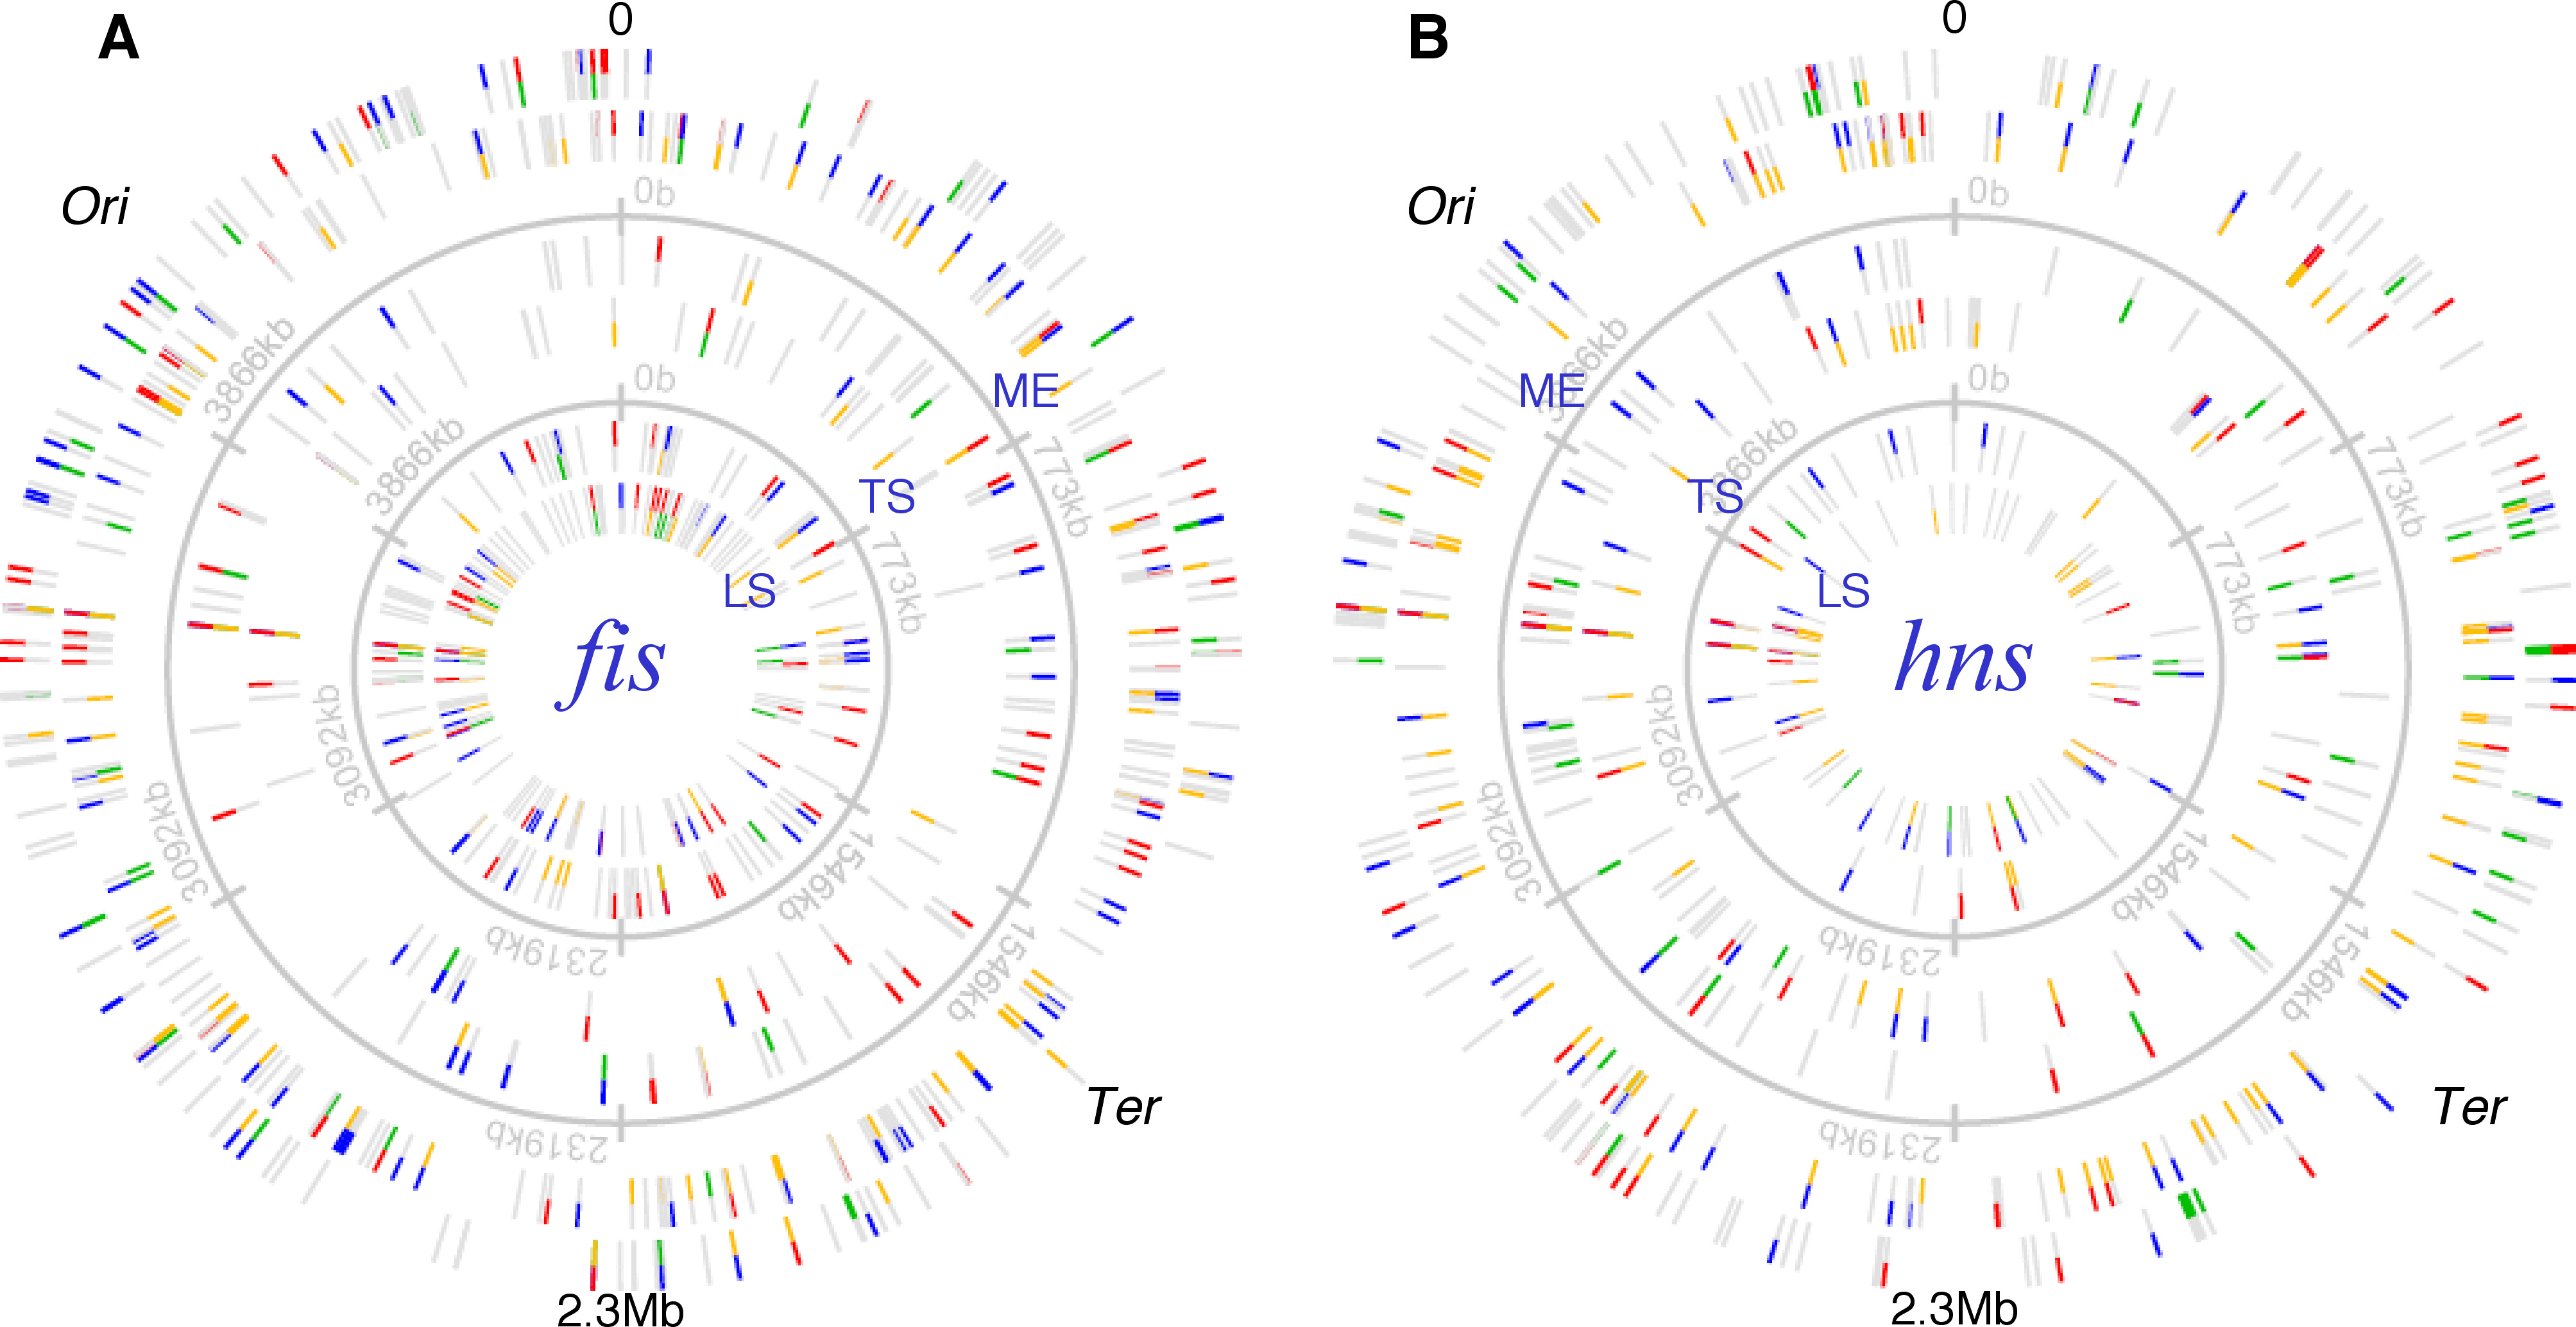
\includegraphics[width=\hsize]{Muskhelishvili/Muskhelishvili-fig1.png}
    \mycaption{\textit{Escherichia coli} genomic wheels showing the differential distributions of four classes of supercoiling-sensitive genes - \textit{Rel} (red), \textit{Hyp} (blue), \textit{Act} (green) and \textit{Rep} (yellow) - among the growth phase-dependent genes (grey) in CSH50 wild type (outer wheels) and mutant (inner wheels) strains. The mutants are lacking global gene regulators, either FIS or H-NS. \textbf{A.} CSH50 wild type vs \textit{fis} mutant. \textbf{B.} CSH50 wild type vs \textit{hns} mutant. \textit{Ori} and \textit{Ter} indicate the origin and terminus of chromosomal replication, respectively. ME, TS and LS indicate the mid-exponential, transition and late stationary growth phases, respectively.}\label{fig:Muskhelishvili-fig1}
   \end{center}
\end{figure}

Publication of a research paper in \textit{EMBO Journal} (together with J�rgen Fritz, Jacobs University, and Andrew Travers, MRC Cambridge) describing for the first time the structural organisation of a transcription initiation complex of major \textit{Escherichia coli} RNA polymerase holoenzyme and a transcriptional activator. The structure described in this article provides a new paradigm for the molecular mechanism of transcriptional regulation of gene expression in bacteria.

A theoretical paper proposing a unified model of molecular mechanisms of gene regulation in Eukaryotes and Prokaryotes has been written (together with my colleague Andrew Travers, MRC Cambridge) and accepted for publication in \textit{EMBO reports}.


A research paper together with Prof. Matthias Ullrich providing new insights into the transcriptional organization of the \textit{algT-muc} gene cluster of \textit{Pseudomonas syringae pv. Glycinea} published in \textit{Journal of Bacteriology}.

A research paper together with colleagues from MRC Cambridge, Ecole Normale Superieure de Cachan, and the University of Camerino describing the identification of the binding site consensus sequence for the global regulator H-NS is in the final stage of preparation. This article provides first clues to the understanding of the mechanistic role of H-NS regulatory protein in virulence gene expression during infectious diseases caused by enteropathogenic \textit{Escherichia coli} and \textit{Salmolla}.


\paragraph{Collaborations}

Bremen Area Collaborations:
\begin{enumerate}
\item {\sl International University Bremen} \\ Prof. K. Brix \\ Confocal microscopy
 \\ Prof. M. Fernandez-Lahore \\Proteomics
 \\ Prof. J. Fritz \\ Atomic force microscopy
 \\ Prof. F.O. Gl�ckner \\ Transcriptomics
 \\ Prof. M.-Th. H�tt \\ Gene regulation networks
\\ Prof. A. Jeltsch \\ Methylation and transcription
 \\ Prof. M. Ullrich \\ Promoter mapping
\\ Prof. M. Zacharias \\ Molecular modeling
\\ Hildegard Meyer-Ortmanns\\ Modeling networks
\end{enumerate}
National \& International Collaborations:
\begin{enumerate}
\item {\sl MRC Cambridge, UK} \\ Dr. A. Travers \\ DNA topology and gene expression
\item {\sl Ecole Normale Superieure de Cachan, France} \\ Dr. M. Buckle \\ DNA binding proteins
\item {\sl Universita di Camerino, Italy} \\ Prof. C. Gualerzi \\ DNA binding proteins
\item {\sl University of Lyon, INSA de Lyon, France} \\ Dr. W. Nasser \\ Regulation of bacterial virulence
\item {\sl National Instutute of Genetics, Mishima, Japan} \\ Prof. N. Shimamoto \\ Regulation of transcription
\end{enumerate}

\paragraph{Grants}
%
\begin{enumerate}
\item Funded by DFG,  \emph{Elucidation of the mechanism of
growth-dependent gene regulation by the \textit{Escherichia coli}
global transcription factor FIS},  grant MU 1549/2-2, (October
2005 - September 2008)
\end{enumerate}

\nocite{Muskhelishvili1,Muskhelishvili2,Muskhelishvili3,Muskhelishvili4,Muskhelishvili5}
